\documentclass[a4paper]{article}
\usepackage{booktabs}
\usepackage{geometry}
\geometry{
  top=1in,
  inner=1in,
  outer=1in,
  bottom=1in,
  headheight=3ex,
  headsep=2ex
}
\usepackage{amssymb,amsmath}
\usepackage{fontspec}
\usepackage[CJKbookmarks, colorlinks, bookmarksnumbered=true,pdfstartview=FitH,linkcolor=black,citecolor=black]{hyperref}
\usepackage{xeCJK}
\usepackage{xltxtra,xunicode}
\usepackage{listings}
\usepackage{xcolor}
\usepackage{array}

\lstset{basicstyle=\footnotesize\ttfamily,        % size of fonts used for the code
        columns=fullflexible,
        numbers=left,
        numberstyle=\tiny,
        keywordstyle=\color{blue},
        stringstyle=\color[rgb]{0,0.6,0},
        commentstyle=\color[cmyk]{1,0,1,0},
        frame=shadowbox,
        escapeinside=``,
        breaklines=true,
        extendedchars=false,
        xleftmargin=2em,xrightmargin=2em, aboveskip=1em,
        tabsize=4, %tab size
        showspaces=false %no space
       }

\newcommand{\tightlist}{
  \setlength{\itemsep}{0pt}\setlength{\parskip}{0pt}}

% font
\setCJKmainfont[AutoFakeBold]{文泉驿微米黑}
\setmainfont[AutoFakeBold]{Segoe UI}
\setromanfont[AutoFakeBold]{Segoe UI}
\setmonofont[Mapping={}]{Monaco}
\linespread{1.2}\selectfont
\XeTeXlinebreaklocale "zh" 

\begin{document}
\title{\Huge 算法导论课程\\ 第二次上机实验报告}
\author { \vspace{12cm} \\ \LARGE 班级:  1413014  \\ \LARGE 姓名:  乔新文   \\ \LARGE 学号:14130140393} 
\date{ \vspace{4cm} 2017.4.12}

\maketitle
\clearpage

\tableofcontents

\clearpage

\section{综述}

本文档将阐述《算法导论》第二次上机实验代码的详细设计及实现。\\

本次上机实验所用代码均为F\#代码,主要算法和辅助定义均包含在SRAlgorithmLib命名空间下AlgorithmLib2.fs所定义的AlgorithmLib2模块中。\\

算法测试驱动部分在Test.fs中Test模块下的P2函数中,整个程序的入口在Program.fs中。\\

本次实验所有代码均运行在.Net Core上,P1.fsproj为项目配置文件,可在安装有.Net Core的环境中在项目文件夹下使用dotnet run命令运行。\\

\section{题目一}

\subsection{题目}

Matrix-chain product

\subsection{实现思路}

使用自底向上的带表格的动态规划方法求解。\\
矩阵链乘最小代价括号化方案的递归求解公式为:

\[m[i,j]=
    \left\{
        \begin{array}{ll}
            0 & ,i=j\\
            min\{ m[i,k]+m[k+1,j]+p_{i-1}p_{k}p_{j} \} & ,i<j
        \end{array}
    \right.
\]

\subsection{实现代码}

计算m[i,j]的代价和最优值m[i,j]对应的分割点k,\\
m中保存了计算矩阵链乘积所需的最少标量乘法次数,s中保存了最优化括号方案的分割点。

\begin{lstlisting}[language=ML]
    let MatrixChainOrder (p: int []) =
        let n = p.Length - 1
        let m = Array2D.create (n + 1) (n + 1) 0.0
        let s = Array2D.create n (n + 1) 0
        for l = 2 to n do
            for i = 1 to n - l + 1 do 
                let j = i + l - 1
                m.[i,j] <- infinity
                for k = i to j - 1 do
                    let q = m.[i,k] + m.[k + 1,j] + float (p.[i - 1] * p.[k] * p.[j])
                    if q < m.[i,j] then
                        m.[i,j] <- q
                        s.[i,j] <- k
        (m,s)
\end{lstlisting}

递归输出最优化括号方案

\begin{lstlisting}[language=ML]
    let rec PrintOptimalParens (s:int [,]) (i:int) (j:int) =
        if i = j then 
            printf "A%i" i
        else 
            printf "("
            PrintOptimalParens s i s.[i,j]
            PrintOptimalParens s (s.[i,j] + 1) j
            printf ")"
\end{lstlisting}

\subsection{算法测试}

\begin{itemize}
\item
    测试样例:
    \begin{itemize}
    \item
        <3, 5, 2, 1,10>
    \item
        <2, 7, 3, 6, 10>
    \item
        <10, 3, 15, 12, 7, 2>
    \item
        <7, 2, 4, 15, 20, 5>
    \end{itemize}
\item
    样例输出
    \begin{itemize}
    \item
        (A1(A2(A3A4)))
    \item
        (((A1A2)A3)A4)
    \item
        (A1(A2(A3(A4A5))))
    \item
        (A1(((A2A3)A4)A5))
    \end{itemize}
\end{itemize}

\section{题目二}

\subsection{题目}

Longest Common Subsequence (LCS)

\subsection{实现思路}
使用自底向上的带表格的动态规划方法求解。\\
LCS的递归求解公式为:
\[c[i,j]=
    \left\{
        \begin{array}{ll}
            0 & ,i=0\ or\ j=0\\
            c[i-1,j-1]+1 & ,i>0\ and \ j>0\ and \ x_{i}=y_{j}\\
            max(c[i,j-1],c[i-1,j]) & ,i>0\ and \ j>0\ and \ x_{i} \neq y_{j}
        \end{array}
    \right.
\]
\subsection{实现代码}

计算LCS长度

\begin{lstlisting}[language=ML]
    let LCSLength (X:string) (Y:string) = 
        let m = X.Length
        let n = Y.Length
        let c = Array2D.create (m + 1) (n + 1) 0
        for i = 0 to m - 1 do
            for j = 0 to n - 1 do
                if X.[i] = Y.[j] then 
                    c.[i + 1,j + 1] <- c.[i,j] + 1
                elif c.[i,j + 1] >= c.[i + 1,j] then
                    c.[i + 1,j + 1] <- c.[i,j + 1]
                else
                    c.[i + 1,j + 1] <- c.[i + 1,j]
        c
\end{lstlisting}

递归的构造LCS

\begin{lstlisting}[language=ML]
    let rec PrintLCS (c : int [,]) (X:string) (Y:string) i j =
        if i = 0 || j = 0 then
            ()
        elif X.[i - 1] = Y.[j - 1] then 
            PrintLCS c X Y (i - 1) (j - 1)
            printf "%c" X.[i - 1]
        elif c.[i - 1,j] >= c.[i,j - 1] then
            PrintLCS c X Y (i - 1) j
        else
            PrintLCS c X Y i (j - 1)
\end{lstlisting}

\subsection{算法测试}

\begin{itemize}
\item
    测试样例:
    \begin{itemize}
    \item
        X: xzyzzyx\\
        Y: zxyyzxz
    \item
        X: ALLAAQANKESSSESFISRLLAIVAD\\
        Y: KLQKKLAETEKRCTLLAAQANKENSNESFISRLLAIVAG
    \end{itemize}
\item
    样例输出
    \begin{itemize}
    \item
        xyzz
    \item
        ALLAAQANKESESFISRLLAIVA
    \end{itemize}
\end{itemize}

\section{题目三}
\subsection{题目}
Max Sum
\subsection{实现思路}
最大和子串存在如下特性
\begin{itemize}
\item
    最大和子串不存在负前缀
\item
    最大和子串不存在负后缀

\end{itemize}
最大和子串的递归求解公式为:
\[m[i]=
    \left\{
        \begin{array}{ll}
            -\infty & ,i<0\\
            x[i] & ,i=0\\
            max(m[i-1]+x[i],x[i]) & ,i>0
        \end{array}
    \right.
\]
\subsection{实现代码}

nowSum保存当前子串(m[i-1]+x[i])的和,maxSum保存具有最大和的历史子串值。
beginIndex,endIndex分别保存当前最大和子串的起始下标和结束下标。

\begin{lstlisting}[language=ML]
    let MaxSum (A:int []) =
        let mutable i,nowSum,maxSum,beginIndex,endIndex = 0,0,0,0,0
        while i < A.Length do
            nowSum <- nowSum + A.[i]
            if nowSum > maxSum then
                maxSum <- nowSum
                endIndex <- i
            if nowSum < 0 then
                nowSum <- 0
                if i + 1 >= A.Length then
                    beginIndex <- i
                else
                    beginIndex <- i + 1
            i <- i + 1
        maxSum,beginIndex,endIndex
\end{lstlisting}

\subsection{算法测试}

\begin{itemize}
\item
    测试样例:
    \begin{itemize}
    \item
        (-2,11,-4,13,-5,-2)
    \end{itemize}
\item
    样例输出
    \begin{itemize}
    \item
        MaxSun:20 \\
        SubString:[|11; -4; 13|]
    \end{itemize}
\end{itemize}
\section{题目四}

\subsection{题目}

Shortest path in multistage graphs. Find the shortest path from 0 to 15 for the following graph.

\subsection{实现思路}
使用自底向上的带表格的动态规划方法求解。\\
最短路径的递归求解公式为:
\[c[i,j,k]=
    \left\{
        \begin{array}{ll}
            0 & ,i=j\\
            g[i,j] & ,k=0\\
            min(c[i,j,k-1],c[i,k,k-1]+c[k,j,k-1]) & ,k>0
        \end{array}
    \right.
\]

\subsection{实现代码}

定义邻接链表的节点元素。

\begin{lstlisting}[language=ML]
    [<Struct>]
    type Node = 
            val ID:int
            val Weight:float
            new (id:int,weight:float) = {ID = id; Weight = weight}
\end{lstlisting}

邻接链表到邻接矩阵的转换方法

\begin{lstlisting}[language=ML]
    let AdjListToAdjMatrix (adjList : Set<Node>[]) =
        let adjMatrix = Array2D.create adjList.Length adjList.Length infinity
        for i = 0 to adjList.Length - 1 do
            adjMatrix.[i,i] <- 0.0
            for j in adjList.[i] do
                adjMatrix.[i,j.ID] <- j.Weight
        
        adjMatrix
\end{lstlisting}

计算所有节点对间最短距离的Floyd算法\\
其中,m保存了节点间的最短距离,s保存了节点对间最短路径上的中间节点

\begin{lstlisting}[language=ML]
    let Floyd (G:float [,]) = 
        let n = Array2D.length1 G
        let m = Array2D.copy G
        let s = Array2D.create n n -1
        for i = 0 to n - 1 do
            for j = 0 to n - 1 do
                for k = 1 to n - 1 do
                    let q = m.[i,k] + m.[k,j]
                    if q < m.[i,j] then
                         m.[i,j] <- q
                         s.[i,j] <- k
        (m,s)
\end{lstlisting}

递归的打印最短路径

\begin{lstlisting}[language=ML]
    let rec PrintFloyd (s:int [,]) (i:int) (j:int) = 
        if i = j then
            printf "%A " i
        elif s.[i,j] = -1 then
            printf "%A %A " i j
        else
            PrintFloyd s i s.[i,j]
            PrintFloyd s s.[i,j] j
\end{lstlisting}

\subsection{算法测试}

\begin{itemize}
\item
    测试样例:
    \begin{itemize}
    \item
        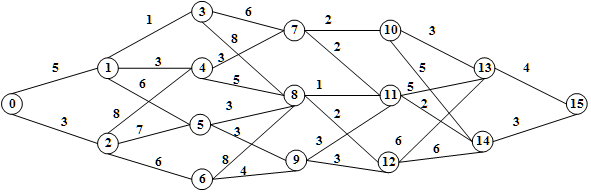
\includegraphics[width=12cm]{2-4.png}
    \end{itemize}
\item
    样例输出
    \begin{itemize}
    \item
        0 1 1 4 4 7 7 11 11 14 14 15
    \end{itemize}
\end{itemize}

\section{题目五}

\subsection{题目}
 Longest Common Substring. 

\subsection{实现思路}
最长公共子串可以看作是最长公共子序列的一个特例。\\
故同样可以按照自底向上的动态规划方法求解。\\
不同的是算法中使用maxLength保存当前最长子串的长度,并在发现有更长的子串的更新maxLength。\\
endIndex用来保存当前最长子串的结束索引,同样的也在发现有更长的子串的更新。

\subsection{实现代码}
\begin{lstlisting}[language=ML]
    let LCSs (X:string) (Y:string) = 
        let m = X.Length
        let n = Y.Length
        let c = Array2D.create (m + 1) (n + 1) 0
        let mutable maxLength = 0
        let mutable endIndex = 0
        for i = 0 to m - 1 do
            for j = 0 to n - 1 do
                if X.[i] = Y.[j] then 
                    c.[i + 1,j + 1] <- c.[i,j] + 1
                    if c.[i + 1,j + 1] > maxLength then
                        maxLength <- c.[i + 1,j + 1]
                        endIndex <- i
        X.[endIndex - maxLength + 1 .. endIndex]
\end{lstlisting}

\subsection{算法测试}
\begin{itemize}
\item
    测试样例:
    \begin{itemize}
    \item
        X: xzyzzyx\\
        Y: zxyyzxz
    \item
        X:MAEEEVAKLEKHLMLLRQEYVKLQKKLAETEKRCALLAAQANKESSSESFISRLLAIVAD\\
        Y:MAEEEVAKLEKHLMLLRQEYVKLQKKLAETEKRCTLLAAQANKENSNESFISRLLAIVAG
    \end{itemize}
\item
    样例输出:
    \begin{itemize}
    \item
        xz
    \item
        MAEEEVAKLEKHLMLLRQEYVKLQKKLAETEKRC
    \end{itemize}
\end{itemize}

\end{document}